\begin{figure*}[htbp]
\centering
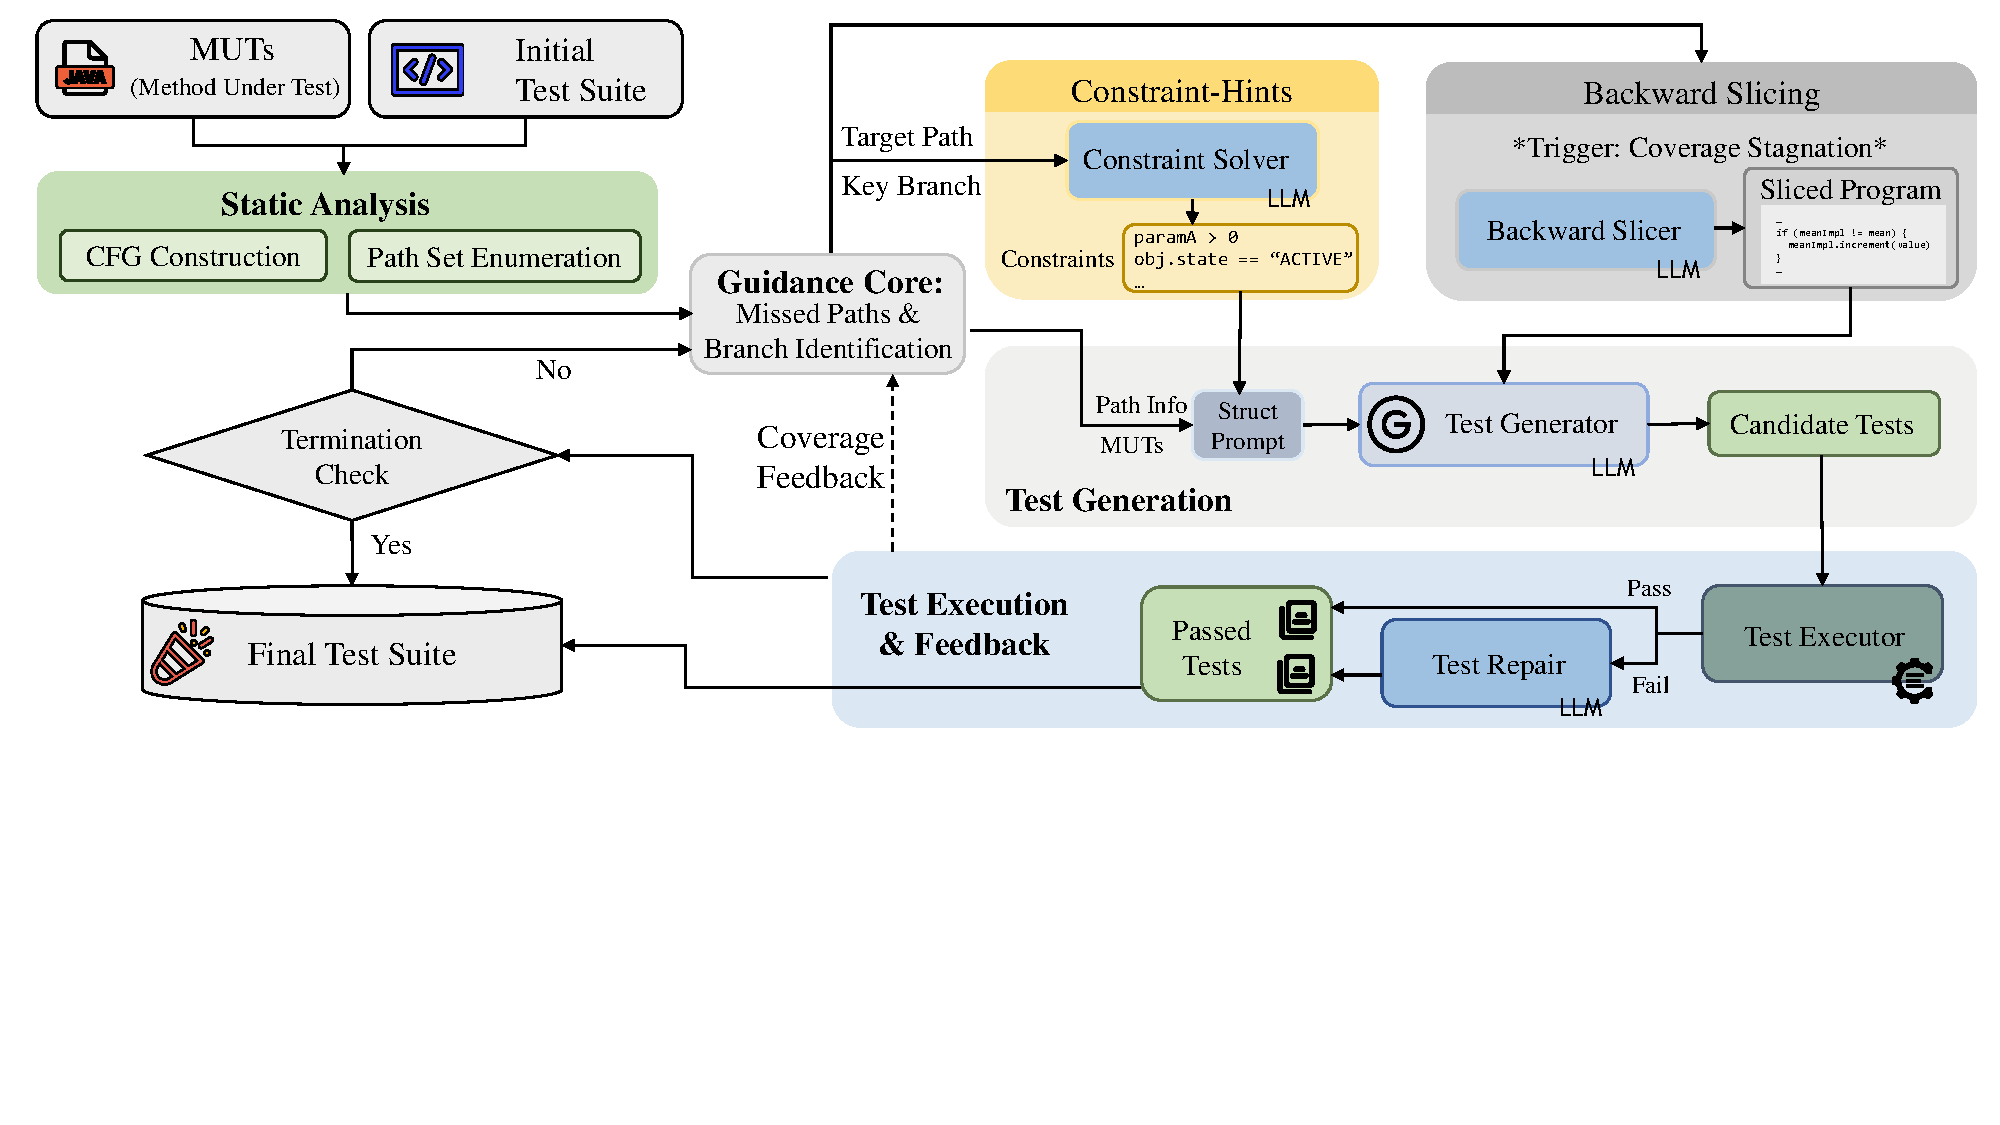
\includegraphics[width=\linewidth]{figures/overview.pdf}
\caption{Overview of the coverage-guided test generation framework.}
\label{fig:overview}
\end{figure*}

\section{Methodology}

\subsection{Overview}

\ourmethod{} is a coverage-guided iterative framework for automated unit test generation, illustrated in Figure~\ref{fig:overview}. Given a method under test, \ourmethod{} first performs an initialization step that extracts project-level dependencies, resolves the required JUnit imports, and seeds the suite with a syntactically valid scaffolding test containing a trivial \texttt{assertTrue(true)} assertion, ensuring a compilable starting point for all subsequent iterations. It then constructs the CFG, enumerates feasible paths, and collects dynamic coverage feedback to identify uncovered branches before entering an iterative refinement loop.

Each iteration begins with path selection, where \textit{Constraint-Hints} analyzes the selected uncovered path and injects explicit branch conditions as structured guidance into the generation prompt. When coverage improvement stagnates, \textit{Backward Slicing} is activated to rebuild the prompt around source-grounded statements and setup actions likely to influence the target branch. The LLM then generates candidate tests against this focused context; passing tests are merged into the suite while failing ones are forwarded to the repair phase. During repair, compiler diagnostics---including error messages and their associated line numbers---are incorporated into the repair prompt, allowing the LLM to precisely locate and correct the offending statements rather than re-generating the test from scratch. Coverage is re-measured at the end of each iteration to drive target selection in the next round. The loop terminates when the coverage target is reached, the iteration budget is exhausted, or coverage fails to improve for a configurable number of consecutive iterations.

\subsection{Constraints-Hints}

\textit{Constraints-Hints} decouples constraint inference from test synthesis. After each test-generation round, \ourmethod{} parses the JaCoCo report to identify missed branches and maps them back to candidate CFG paths. For a selected path $\pi$, the first missed branch $b^*$ is treated as the immediate coverage obstacle, and the LLM is asked to produce sufficient conditions for reaching it rather than a full symbolic solution.

Let $\pi=\langle b_1,b_2,\ldots,b_k\rangle$ denote the branch decisions along a target CFG path. Covering $\pi$ requires an input assignment $\mathbf{x}^*$ that satisfies:
\begin{equation}
\mathbf{x}^* \in \mathcal{F}(\pi) =
\left\{
\mathbf{x} \mid
b_1(\mathbf{x}) \wedge b_2(\mathbf{x}) \wedge \cdots \wedge b_k(\mathbf{x})
\right\}.
\end{equation}
Rather than solving $\mathcal{F}(\pi)$ exactly, which is brittle under complex object states and indirect calls~\cite{baldoni2018, cadar2008klee}, \ourmethod{} approximates it as a lightweight set of interpretable hints $\mathcal{C}(\pi)$. The prompt includes the source code, the selected CFG path, and $b^*$; the output describes variable relations, nullness requirements, object states, and setup actions such as setter or factory calls. These hints are appended to the test-generation prompt, turning an opaque coverage target into explicit guidance about what the generated test must satisfy.

\subsection{Branch-Aligned Context Slicing}

Coverage improvement does not always progress smoothly: certain branches remain persistently uncovered even after multiple generate--execute--repair iterations. In such cases, continuing to expose the same full method body often repeats the same failure. \ourmethod{} therefore performs \emph{slicing-inspired branch context construction}: it rebuilds the prompt around source-grounded statements and setup actions that are likely to affect a specific uncovered branch.

This step is inspired by backward slicing, but it is not intended to replace classical SDG- or PDG-based slicing. Classical static slicers~\cite{weiser1984, ferrante1987}, such as JavaSlicer~\cite{JavaSlicer}, aim to compute sound dependence closures over complete and well-resolved programs. Our setting is different: the generation prompt is restricted to the declaring class source and imports, while branch reachability may depend on object states established through setters, factory methods, or framework initialization logic. We therefore use slicing as a prompt-alignment operation rather than as a formal dependence-analysis claim. The produced context is approximate, source-grounded, and validated only through downstream compilation, execution, and coverage feedback.

\textit{Branch criterion.}
Let $b^*$ denote the first uncovered branch on a selected path, with predicate $P$ located at source line $\ell$ in the focal method $M$. We define the branch-context criterion as:
\begin{equation}
C = \langle \ell, P, V(P) \rangle,
\end{equation}
where $V(P)$ contains the variables, fields, and receiver objects referenced by the predicate. When $P$ invokes helper methods or accesses object fields, $V(P)$ is expanded with receiver state and field accesses that are visible within the declaring class. This criterion makes the target of context reduction explicit: the context is constructed for a concrete uncovered branch, not for the method as a whole.

\textit{Context extraction.}
Given $C$, the slicer LLM receives the declaring class source with line numbers, the focal method, the target predicate and line number, and the signatures or bodies of methods in the declaring class that are referenced by the focal method. The model is prompted to return a structured tuple:
\[
\langle \mathit{stmts}, \mathit{states}, \mathit{setups}, \mathit{rationale} \rangle,
\]
where $\mathit{stmts}$ are source-grounded statements that may data- or control-influence $P$, $\mathit{states}$ describe object states required at $\ell$, $\mathit{setups}$ list candidate calls such as setters or factory methods needed to establish those states, and $\mathit{rationale}$ briefly explains the dependency chain.

To reduce hallucination, \ourmethod{} validates the returned statements against the numbered source code and discards entries whose line numbers or text do not match the declaring class. The resulting context is therefore not assumed to be sound, complete, or minimal; it is a branch-focused prompt artifact used to guide the next generation attempt.

\textit{Use in test generation.}
The validated tuple is supplied to the test-generation prompt as focused branch context. Generated tests are compiled, executed, and measured using the same validation pipeline as regular candidates. A slice affects the final suite only through tests that compile, pass, and improve or preserve coverage; incorrect or incomplete contexts are filtered by execution feedback rather than being accepted as program-analysis results.

\subsection{Iterative Workflow of \ourmethod{}}

\begin{algorithm}[t]
\small
\caption{Iterative Test Generation with Constraints-Hints and Backward Slicing}
\label{alg:main}
\SetAlgoLined
\KwIn{$\textit{src}$: source file, $\textit{suite}$: initial test suite (possibly empty)}
\KwOut{Augmented test suite with improved coverage}

$\textit{deps} \leftarrow \textsc{ExtractDeps}()$\;
$\textit{cfg}, \textit{methodDict} \leftarrow \textsc{BuildCFG}(\textit{src})$\;
$\textit{noIncr} \leftarrow 0$, \quad $\textit{iter} \leftarrow 0$\;
$\textit{cov}, \textit{missed} \leftarrow \textsc{RunCoverage}(\textit{suite})$\;

\While{$\textit{iter} < \textit{maxIter}$ \textbf{and} $\textit{noIncr} < \Lambda$ \textbf{and} $\textit{cov} < \tau$}{

    \tcp{Path selection and prompt construction}
    \eIf{$\textit{cov} = 0$ \textbf{or} $\textit{iter} = 0$}{
        $\textit{prompt} \leftarrow \textsc{BuildBaselinePrompt}(\textit{src}, \textit{suite}, \textit{deps})$\; \tcp*[r]{baseline prompt}
    }{
        $\Pi \leftarrow \textsc{SelectPaths}(\textit{cfg}, \textit{methodDict}, \textit{missed})$\;
        $\mathcal{C} \leftarrow \emptyset$\;
        \ForEach{path $\pi \in \Pi$}{
            $b^* \leftarrow \textsc{FirstUncoveredBranch}(\pi, \textit{missed})$\;
            $\mathcal{C}(\pi) \leftarrow \textsc{ConstraintSolver}(\textit{src}, \pi, b^*)$\; \tcp*[r]{Constraints-Hints}
        }
        $\textit{prompt} \leftarrow \textsc{BuildPrompt}(\textit{src}, \textit{suite}, \textit{deps}, \Pi, \mathcal{C})$\;
    }

    \tcp{Test generation}
    $\mathcal{T} \leftarrow \textsc{GenerateTests}(\textit{prompt})$\;

    \tcp{Backward slicing for stubborn uncovered paths}
    \If{$\textit{noIncr} \geq \beta \cdot \Lambda$}{
        $\textit{slices} \leftarrow \textsc{BackwardSlicer}(\textit{src}, \textit{missed})$\;
        $\mathcal{T} \leftarrow \mathcal{T} \cup \textsc{GenerateFromSlices}(\textit{slices}, \textit{suite}, \textit{deps})$\;
    }

    \tcp{Validation and repair}
    $\textit{failed} \leftarrow \{\}$\;
    \ForEach{$t \in \mathcal{T}$}{
        \lIf{$\textsc{ValidateTest}(t, \textit{suite})$}{$\textit{suite} \leftarrow \textit{suite} \cup \{t\}$}
        \lElse{$\textit{failed} \leftarrow \textit{failed} \cup \{t\}$}
    }
    \If{$\textit{failed} \neq \emptyset$}{
        $\textit{suite} \leftarrow \textit{suite} \cup \textsc{RepairAndValidate}(\textit{failed}, \textit{src}, \textit{suite}, \textit{deps})$\;
    }

    \tcp{Coverage update and termination check}
    $(\textit{cov}',\, \textit{missed}') \leftarrow \textsc{RunCoverage}(\textit{suite})$\;
    \lIf{$\textit{cov}' > \textit{cov}$}{$\textit{noIncr} \leftarrow 0$}
    \lElse{$\textit{noIncr} \leftarrow \textit{noIncr} + 1$}
    $\textit{cov} \leftarrow \textit{cov}'$, \quad
    $\textit{missed} \leftarrow \textit{missed}'$, \quad
    $\textit{iter} \leftarrow \textit{iter} + 1$\;
}

\Return $\textit{suite}$\;
\end{algorithm}

The complete workflow of \ourmethod{} is formalized in Algorithm~\ref{alg:main}. The framework accepts the source file and an initial test suite as input, and iteratively generates, validates, and repairs tests until a coverage target is met or a termination condition is triggered.


{\em Initialization.}
The framework extracts test-scope dependencies, constructs the CFG and method dictionary from the source file, deriving branch sequences and inter-procedural dependency information to bootstrap Constraint-Hints and Backward Slicing respectively. Baseline coverage is then measured on the initial suite (lines 1--4), providing the missed-branch information that drives subsequent path selection.

{\em Path selection with Constraints-Hints.}
At each non-initial iteration, \textsc{SelectUncoveredPaths} identifies CFG paths that intersect with missed lines or branches and records the number of previous hint-generation attempts for each path in $\textit{pathHistory}$ (line 8). Paths with fewer attempts are prioritized, subject to coverage impact, so that \ourmethod{} explores under-tried uncovered paths instead of repeatedly targeting the same stalled path. For each selected path $\pi$, the constraint solver derives $\mathcal{C}(\pi)$ by analyzing the branch sequence up to the first uncovered predicate $b^*$, and these conditions are embedded into the generation prompt (lines 9--13).

{\em Backward slicing.}
When $\textit{noIncr} \geq \beta \cdot \Lambda$, indicating a coverage plateau, the backward slicer is invoked on the remaining missed code segments. It returns a source-grounded branch context---relevant statements, required object states, and setup actions---which is used to construct an additional batch of targeted tests $\mathcal{T}_s$ (lines 16--19).

{\em Validation and repair.}
Each generated test is individually inserted into the suite and executed. Failing tests are collected with their error messages and forwarded to the repair phase, which re-invokes the LLM with failure feedback to produce corrected versions. Successfully validated repaired tests are also incorporated into the suite (lines 21--32).

{\em Termination.}
The loop exits when the coverage target $\tau$ is reached, the maximum iteration count $\textit{maxIter}$ is exhausted, or coverage fails to improve for $\Lambda$ consecutive iterations.
